%-*- coding: utf-8 -*-
\documentclass[dvipsk]{beamer}
\usepackage{pgfpages}
\usepackage{moreverb,array}
%\usetheme{Malmoe}
%\usetheme{Goettingen} %7 8 9
%\usetheme{Darmstadt}% 1, 2, 3
%\usetheme{Boadilla}
%\usetheme{CambridgeUS}%4, 5 6 
%
\usetheme{AnnArbor} %10
%\usetheme{Marburg}
\iffalse\else
\renewcommand{\familydefault}{\sfdefault}
\renewcommand{\kanjifamilydefault}{\gtdefault}
\setbeamerfont{title}{size=\Large,series=\bfseries}%,color=white}
\setbeamerfont{frametitle}{size=\large,series=\bfseries}
\setbeamerfont{beamergotobutton}{size=\Large}
%\setbeamercolor{frametitle}{fg=yellow}
\setbeamertemplate{frametitle}[default][center]
%\addtobeamertemplate{footline}{}{\insertframenumber/\inserttotalframenumber}
\usefonttheme{professionalfonts}
\fi
%\iftrue
\title{ソフトウェア開発\\第14回目授業}
\author{平野 照比古}
\institute{}
\date{2016/1/15}
\newtheorem{Prob}{解説}
\newcommand{\Elm}[1]{\texttt{<#1>}}
\setbeamercovered{transparent}

\newcommand{\DOMM}{\texttt}
\newcommand{\Event}{\texttt}
\newcommand{\DOMP}{\texttt}
\newcommand{\DOM}{\texttt{DOM}}
\newcommand{\keyitem}{\relax}
\newcommand{\HTML}{HTML文書}
\begin{document}
\frame{\maketitle}
\section{jQueryのコードを読む}
\begin{frame}[containsverbatim]
 \frametitle{jQueryファイルの違い}
\begin{itemize}
 \item jQueryのソースファイルには\texttt{jQuery-<Version No>.js}と
\texttt{jQuery-<Version No>.min.js}の2種類が存在
 \item \texttt{jQuery-<Version No>.min.js}は\texttt{jQuery-<Version No>.js}から
コメントや、空白を取り除き、変数名を短いものに置き換えるという操作を行っ
て、ファイルサイズを小さくしたもの
\end{itemize}
\end{frame}
\begin{frame}[containsverbatim]
 \frametitle{jQuery のソースコード(1)}
 {\footnotesize
\begin{verbatim}
/*!
 * jQuery JavaScript Library v1.11.3
 * http://jquery.com/
 *
 * Includes Sizzle.js
 * http://sizzlejs.com/
 *
 * Copyright 2005, 2014 jQuery Foundation, Inc. and other contributors
 * Released under the MIT license
 * http://jquery.org/license
 *
 * Date: 2015-04-28T16:19Z
 */
 }
\end{verbatim}
 }
\end{frame}
\begin{frame}[containsverbatim]
 \frametitle{jQuery のソースコード(2)}
 {\tiny
\begin{verbatim}
(function( global, factory ) {
  if ( typeof module === "object" && typeof module.exports === "object" ) {
    // For CommonJS and CommonJS-like environments where a proper window is present,
    // execute the factory and get jQuery
    // For environments that do not inherently posses a window with a document
    // (such as Node.js), expose a jQuery-making factory as module.exports
    // This accentuates the need for the creation of a real window
    // e.g. var jQuery = require("jquery")(window);
    // See ticket #14549 for more info
    module.exports = global.document ?
      factory( global, true ) :
      function( w ) {
        if ( !w.document ) {
          throw new Error( "jQuery requires a window with a document" );
        }
        return factory( w );
      };
  } else {
    factory( global );
  }
// Pass this if window is not defined yet
}(typeof window !== "undefined" ? window : this, function( window, noGlobal ) {
\end{verbatim}
 }
\end{frame}
\begin{frame}[containsverbatim]
 \frametitle{jQuery のソースコード(3)}
 {\footnotesize
\begin{verbatim}
	// Can't do this because several apps including ASP.NET trace
// the stack via arguments.caller.callee and Firefox dies if
// you try to trace through "use strict" call chains. (#13335)
// Support: Firefox 18+
//
var deletedIds = [];
var slice = deletedIds.slice;
var concat = deletedIds.concat;
var push = deletedIds.push;
var indexOf = deletedIds.indexOf;
var class2type = {};
var toString = class2type.toString;
var hasOwn = class2type.hasOwnProperty;
var support = {};
\end{verbatim}
 }
\end{frame}
\begin{frame}[containsverbatim]
 \frametitle{jQuery のソースコード(tiny)}
 {\footnotesize
\begin{verbatim}
var
  version = "1.11.3",
  // Define a local copy of jQuery
  jQuery = function( selector, context ) {
    // The jQuery object is actually just the init constructor 'enhanced'
    // Need init if jQuery is called (just allow error to be thrown if not included)
    return new jQuery.fn.init( selector, context );
  },
  // Support: Android<4.1, IE<9
  // Make sure we trim BOM and NBSP
  rtrim = /^[\s\uFEFF\xA0]+|[\s\uFEFF\xA0]+$/g,
  // Matches dashed string for camelizing
  rmsPrefix = /^-ms-/,
  rdashAlpha = /-([\da-z])/gi,
  // Used by jQuery.camelCase as callback to replace()
  fcamelCase = function( all, letter ) {
    return letter.toUpperCase();
  };
\end{verbatim}
 }
\end{frame}
\begin{frame}[containsverbatim]
 \frametitle{jQuery 1.12.2.jsのソース}
 \begin{itemize}
  \item このリストでは詳細なコメントが付いていて比較的読みやすい。
  \item コメントを見るとクロスブラウザ対策が行われていることも見て取れる。
  \item ソースコードの最小化のテクニックとしてグローバルなオブジェクトを短い変数
名で置き換える
  \item 冒頭の定義された関数
の引数に、関数を渡している。その関数の仮引数は\texttt{window}となってい
る。これにより、開発時はわかりやすい変数名が使えるメリットがある。
 \end{itemize}
\end{frame}
\begin{frame}[containsverbatim]
\frametitle{短縮化のリスト}
{\scriptsize
\begin{verbatim}
/*! jQuery v1.11.3 | (c) 2005, 2015 jQuery Foundation, Inc. | jquery.org/license */
!function(a,b){"object"==typeof module&&"object"==typeof
    module.exports?module.exports=a.document?b(a,!0):function(a){if(!a.document)throw
    new Error("jQuery requires a window with a document");
  return b(a)}:b(a)}
    ("undefined"!=typeof window?window:this,function(a,b){
      var c=[],d=c.slice,e=c.concat,f=c.push,g=c.indexOf,h={},i=h.toString,
  j=h.hasOwnProperty,k={},l="1.11.3",
  m=function(a,b){return new  m.fn.init(a,b)},
  n=/^[\s\uFEFF\xA0]+|[\s\uFEFF\xA0]+$/g,o=/^-ms-/,
  p=/-([\da-z])/gi,q=function(a,b){return b.toUpperCase()};
\end{verbatim}
}
\end{frame}
\begin{frame}[containsverbatim]
\frametitle{短縮化の方法}
\begin{itemize}
 \item 各関数内で変数名は1文字から始めている。
 \item 関数の仮引数も\texttt{a}から付け直している。
 \item JavaScriptの固有の関数は当然のことながら変換されていない。
 \item このライブラリーは一つの関数を定義して、その場で実行している。14
       行目の\texttt{function()}の前に\texttt{(}がついている。
 \item 短縮化されたコードではこの部分が\texttt{!function()}となっている。
       関数オブジェクトを演算の対象とすることで実行する。
 \item そのほかにもキーワード\texttt{true}の代わりに\texttt{!0}としてい
       る。
 \item \texttt{if()\{\}else\{\}}構文は\texttt{?}に置き換えている。
\end{itemize}
\end{frame}
\section{JavaScriptファイルの短縮化の例}
\begin{frame}[containsverbatim]
 \frametitle{JavaScriptファイルの短縮化ツール}
 JavaScriptの短縮化ツールとして、Googleが提供する
 Closure Compiler を紹介する。
 このサービスは次のように説明されている。
\begin{quotation}
 The Closure Compiler is a tool for making JavaScript download and run
 faster. It is a true compiler for JavaScript. Instead of compiling from
 a source language to machine code, it compiles from JavaScript to
 better JavaScript. It parses your JavaScript, analyzes it, removes dead
 code and rewrites and minimizes what's left. It also checks syntax,
 variable references, and types, and warns about common JavaScript
 pitfalls. 
\end{quotation}
\end{frame}
\begin{frame}[containsverbatim]
\frametitle{Closure Compiler の使い方}
使い方については次のように書かれている。
\begin{quotation}
 You can use the Closure Compiler as:

\begin{itemize}
 \item An open source Java application that you can run from the command
			 line.
 \item A simple web application.
 \item A RESTful API.
\end{itemize}
To get started with the compiler, see "How do I start" below.
\end{quotation}
ここでは2番目にある Web アプリケーションで行う。
\end{frame}
\begin{frame}[containsverbatim]
\frametitle{Closure Compiler の Web サイト}
 サイトは\texttt{http://closure-compiler.appspot.com/home}
 \begin{figure}[ht]
	\begin{center}
	 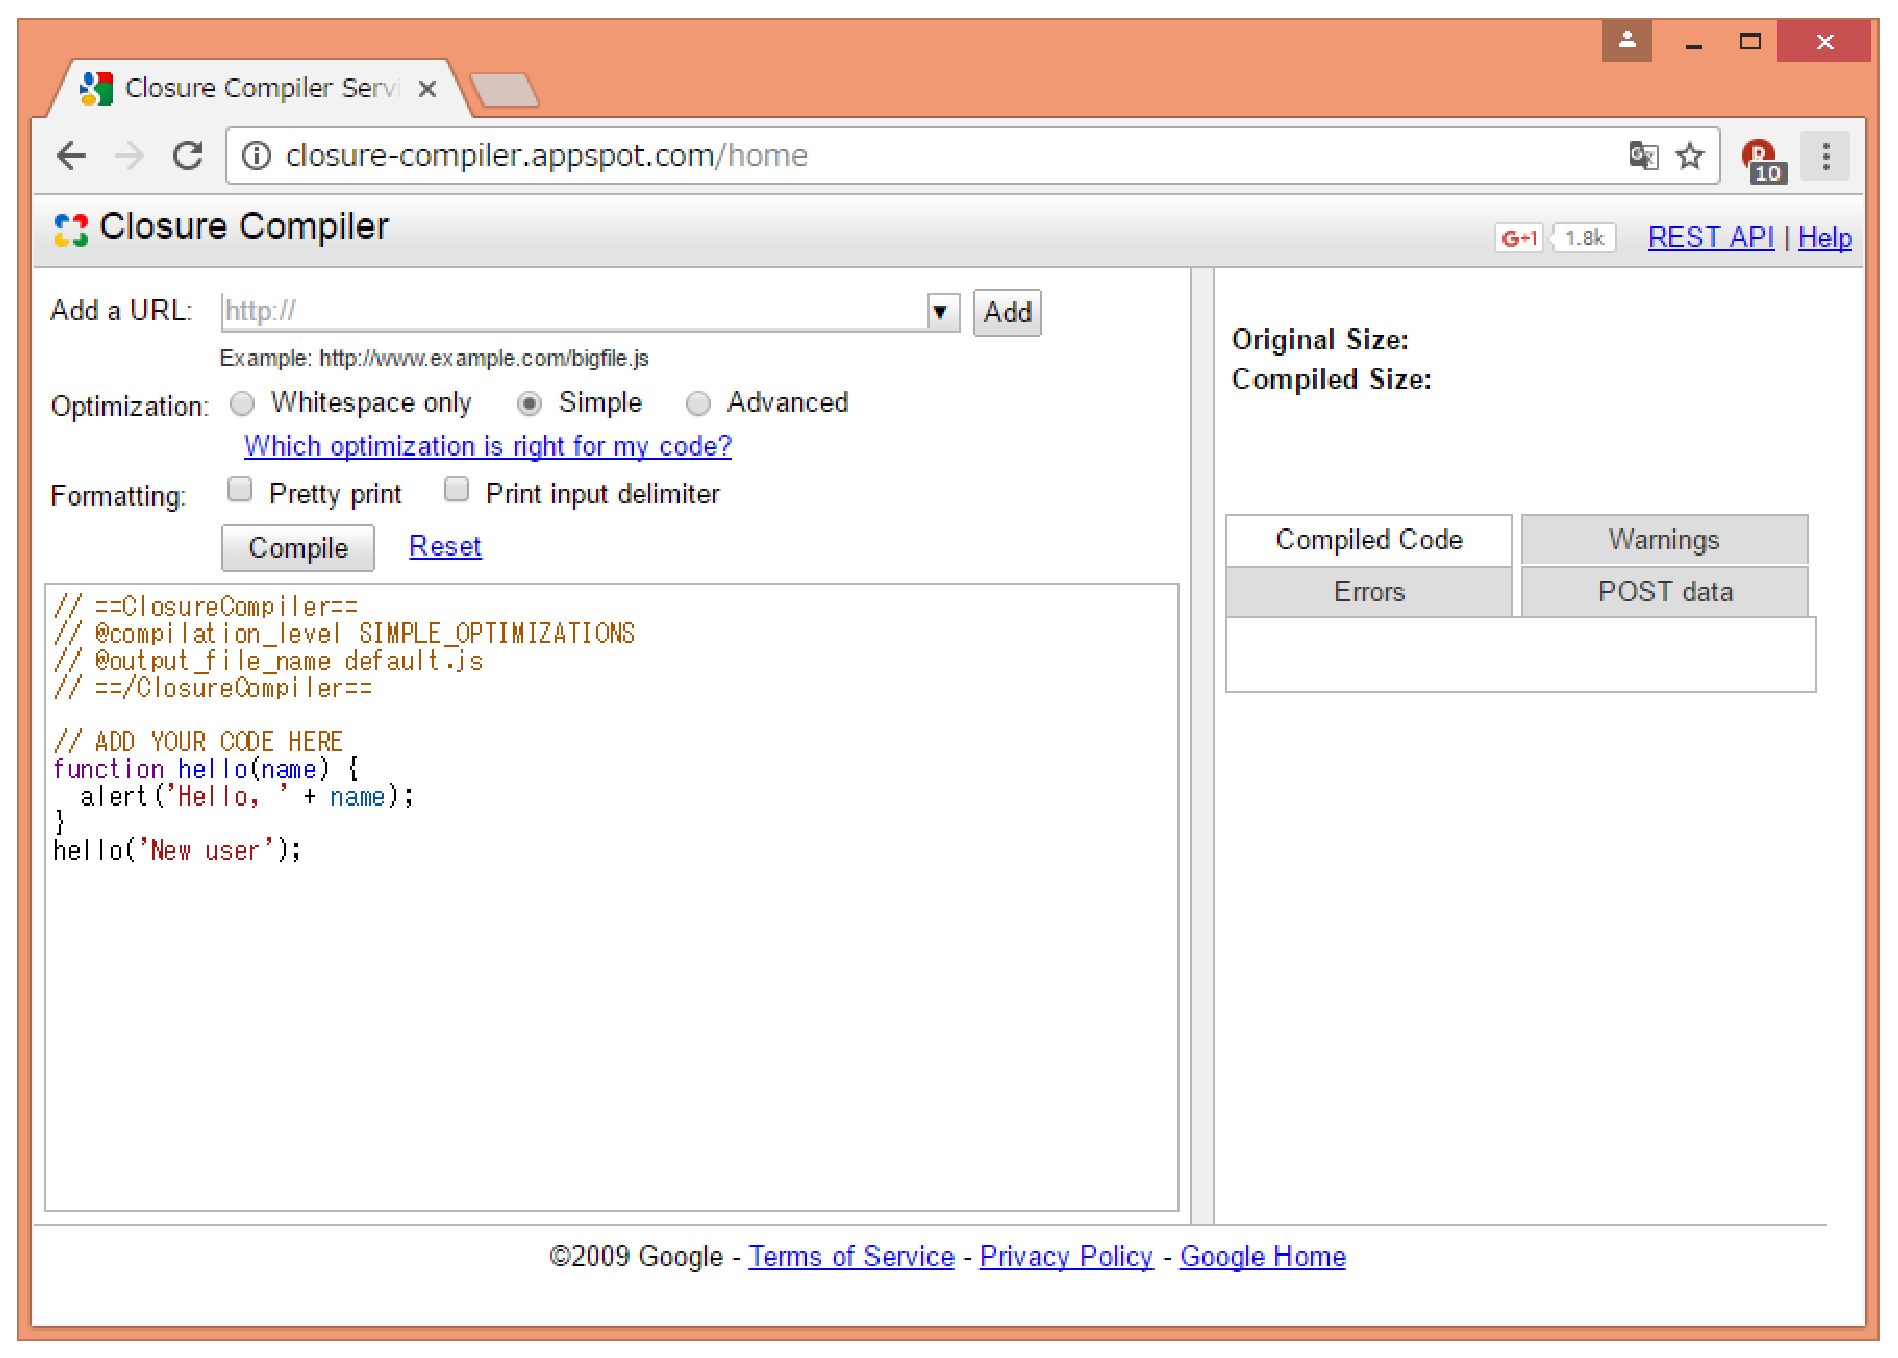
\includegraphics[width=1\textwidth]{../10-01closur-compiler-home.eps}
	\end{center}
 \caption{Closure Compiler のホームページ}\label{closure-compiler}
 \end{figure}
 左側のテキストボックスにコードを張り付けて、「Compile」のボタンを押せば
 よい。
\end{frame}
\section{短縮化の例}
\begin{frame}[containsverbatim]
 \frametitle{短縮化の例}
 使用するファイルは9回目の授業で用いた\texttt{event.js}
 \begin{figure}[ht]
	\begin{center}
	 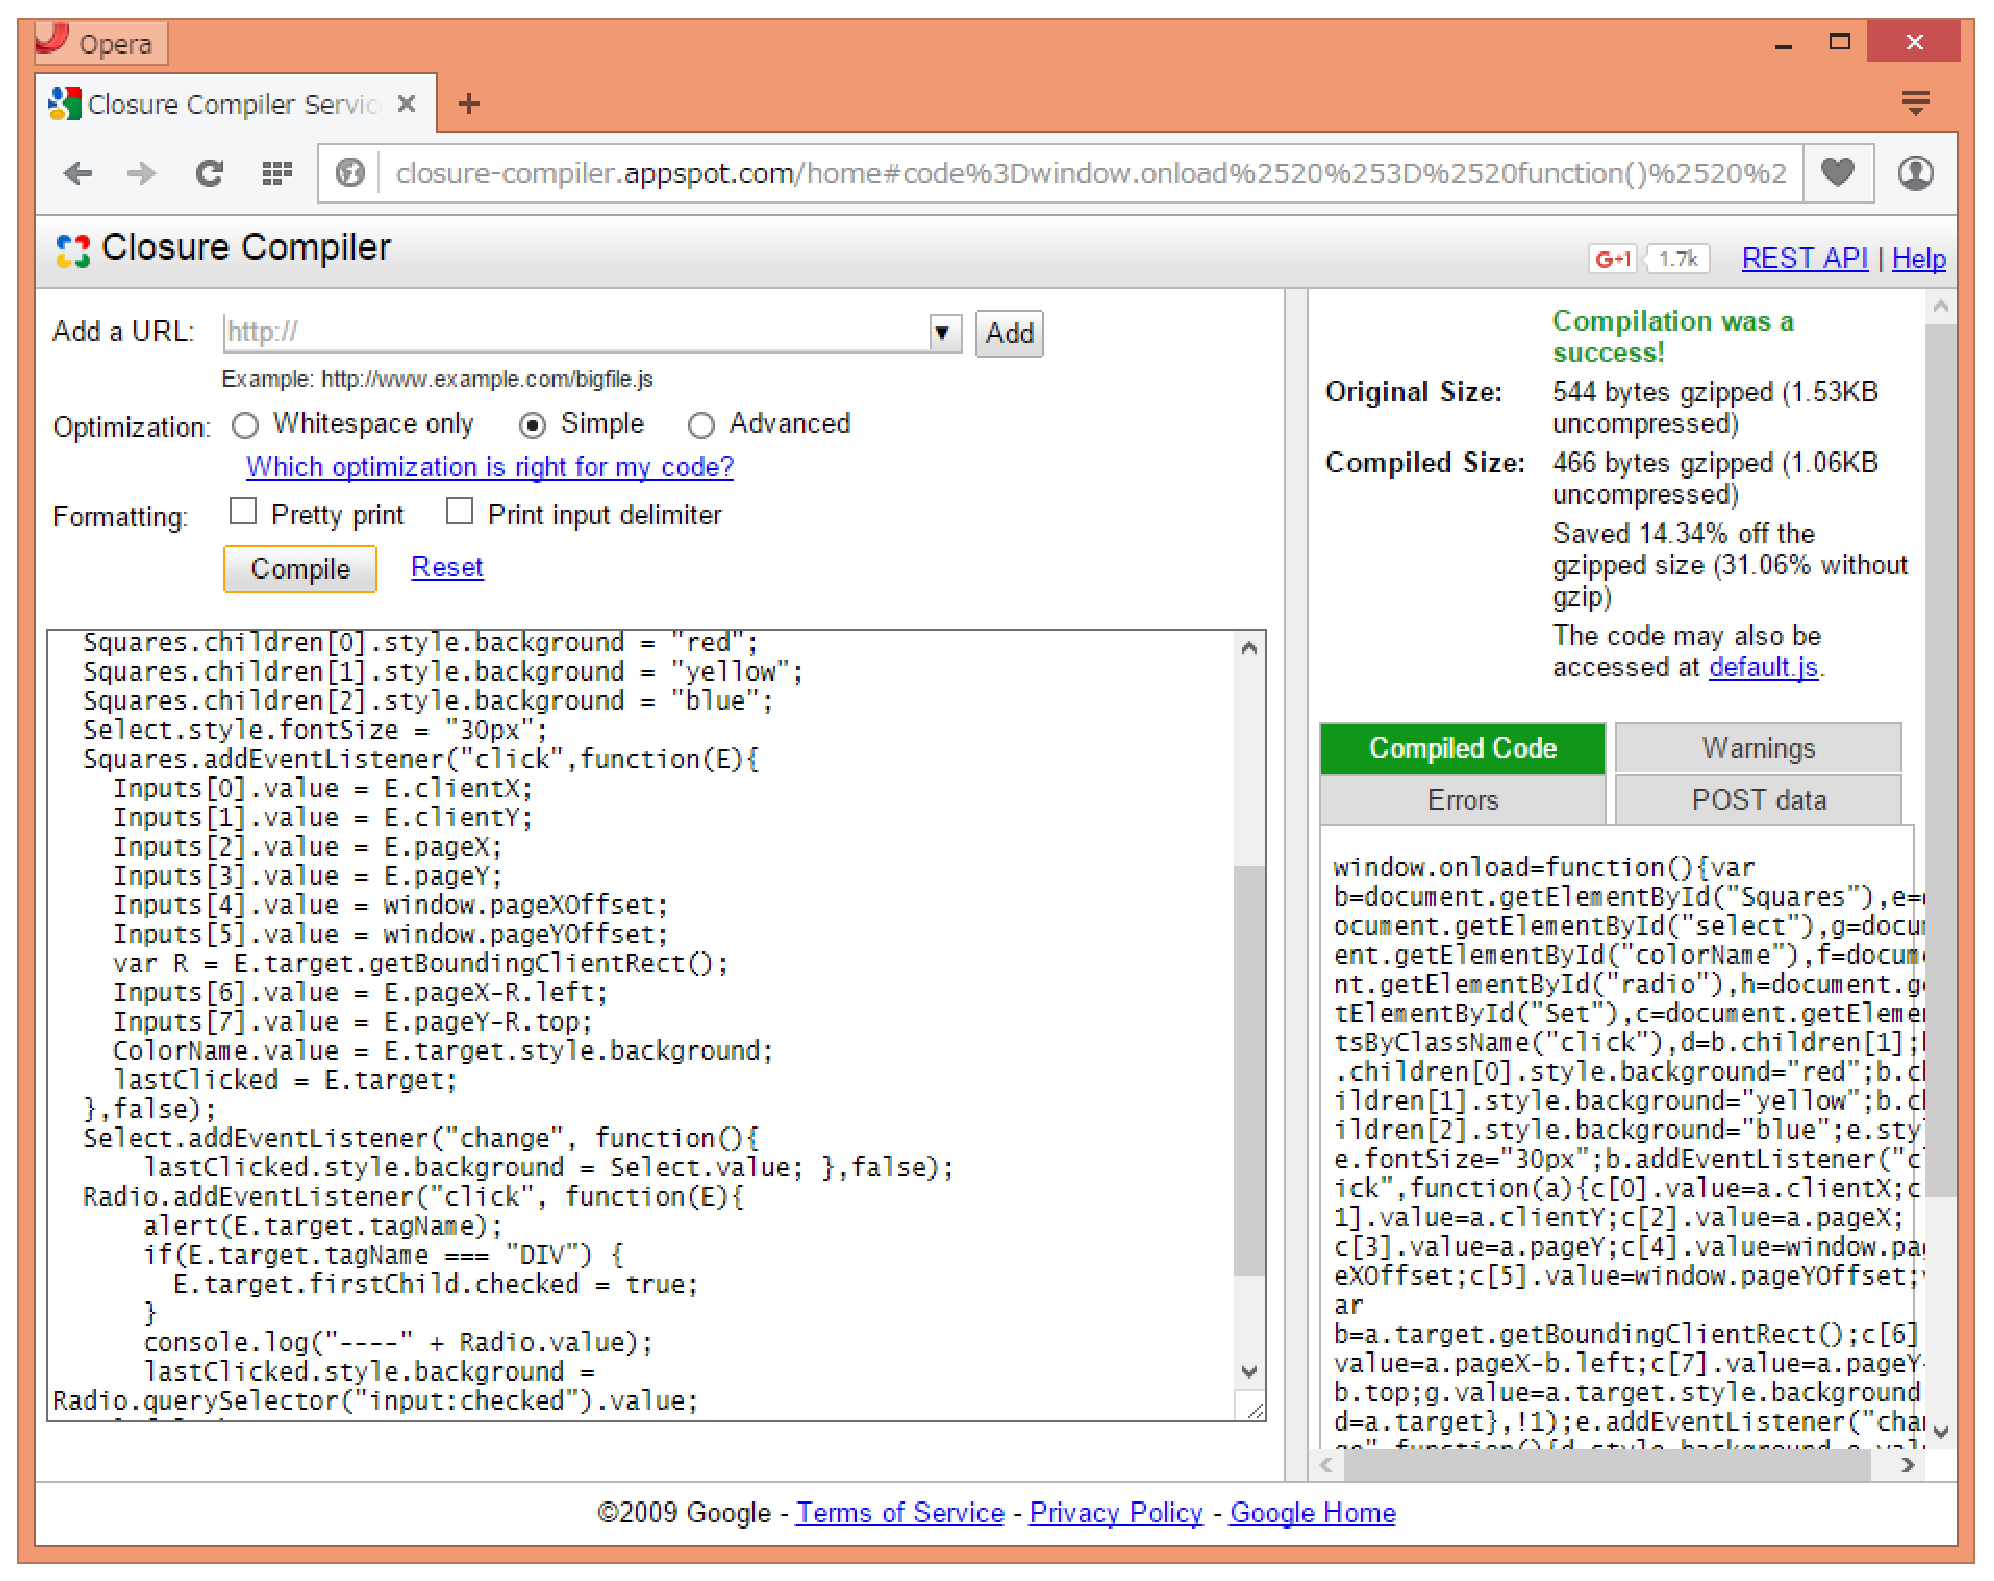
\includegraphics[width=1\textwidth]{../10-01closur-compiler-res01.eps}
	\end{center}
 \caption{Closure Compiler の結果}\label{closure-compiler-res01}
 \end{figure}
\end{frame}
\begin{frame}[containsverbatim]
\frametitle{短縮化の結果(1)}
 画面の右のほうで、元のファイルの大きさが1.53KBであったのに対し、短縮化
 の結果が1.06KBとなったことがわかる。
\end{frame}
\begin{frame}[containsverbatim]
 \frametitle{短縮化の詳細}
 {\footnotesize
\begin{verbatim}
window.onload=function(){var b=document.getElementById("Squares"),
  e=document.getElementById("select"),
  g=document.getElementById("colorName"),
  f=document.getElementById("radio"),
  h=document.getElementById("Set"),
  c=document.getElementsByClassName("click"),
  d=b.children[1];
  b.children[0].style.background="red";
  b.children[1].style.background="yellow";
  b.children[2].style.background="blue";
  e.style.fontSize="30px";
\end{verbatim}
 }
\end{frame}
\begin{frame}[containsverbatim]
 \frametitle{短縮化の結果(2)}
 {\footnotesize
\begin{verbatim}
  b.addEventListener("click",function(a){
    c[0].value=a.clientX;
    c[1].value=a.clientY;
    c[2].value=a.pageX;
    c[3].value=a.pageY;
    c[4].value=window.pageXOffset;
    c[5].value=window.pageYOffset;
    var b=a.target.getBoundingClientRect();
    c[6].value=a.pageX-b.left;
    c[7].value=a.pageY-b.top;
    g.value=a.target.style.background;
    d=a.target
  },!1);
\end{verbatim}
 }
\end{frame}
\begin{frame}[containsverbatim]
 \frametitle{短縮化の結果(3)}
 {\footnotesize
\begin{verbatim}
  e.addEventListener("change",function(){
    d.style.background=e.value},!1);
  f.addEventListener("click",function(a){
    alert(a.target.tagName);
  "DIV"===a.target.tagName&&(a.target.firstChild.checked=!0);
  console.log("----"+f.value);
  d.style.background=f.querySelector("input:checked").value
  },!1);
  h.addEventListener("click",function(){
    d.style.background=g.value},!1)};
\end{verbatim}
 }
 \begin{itemize}
	\item  \texttt{if}文であったものが論理式の\verb+&&+で置き換えられてい
				 る。
	\item \texttt{document.getElementById}などはそのまま短縮化、共通化さ
れていない。
 \end{itemize}

\end{frame}
\begin{frame}[containsverbatim]
 \frametitle{\texttt{document.getElementById}を減らす}
 単純に関数を置き換えただけではうまくいかない。
  \begin{figure}[ht]
	\begin{center}
	 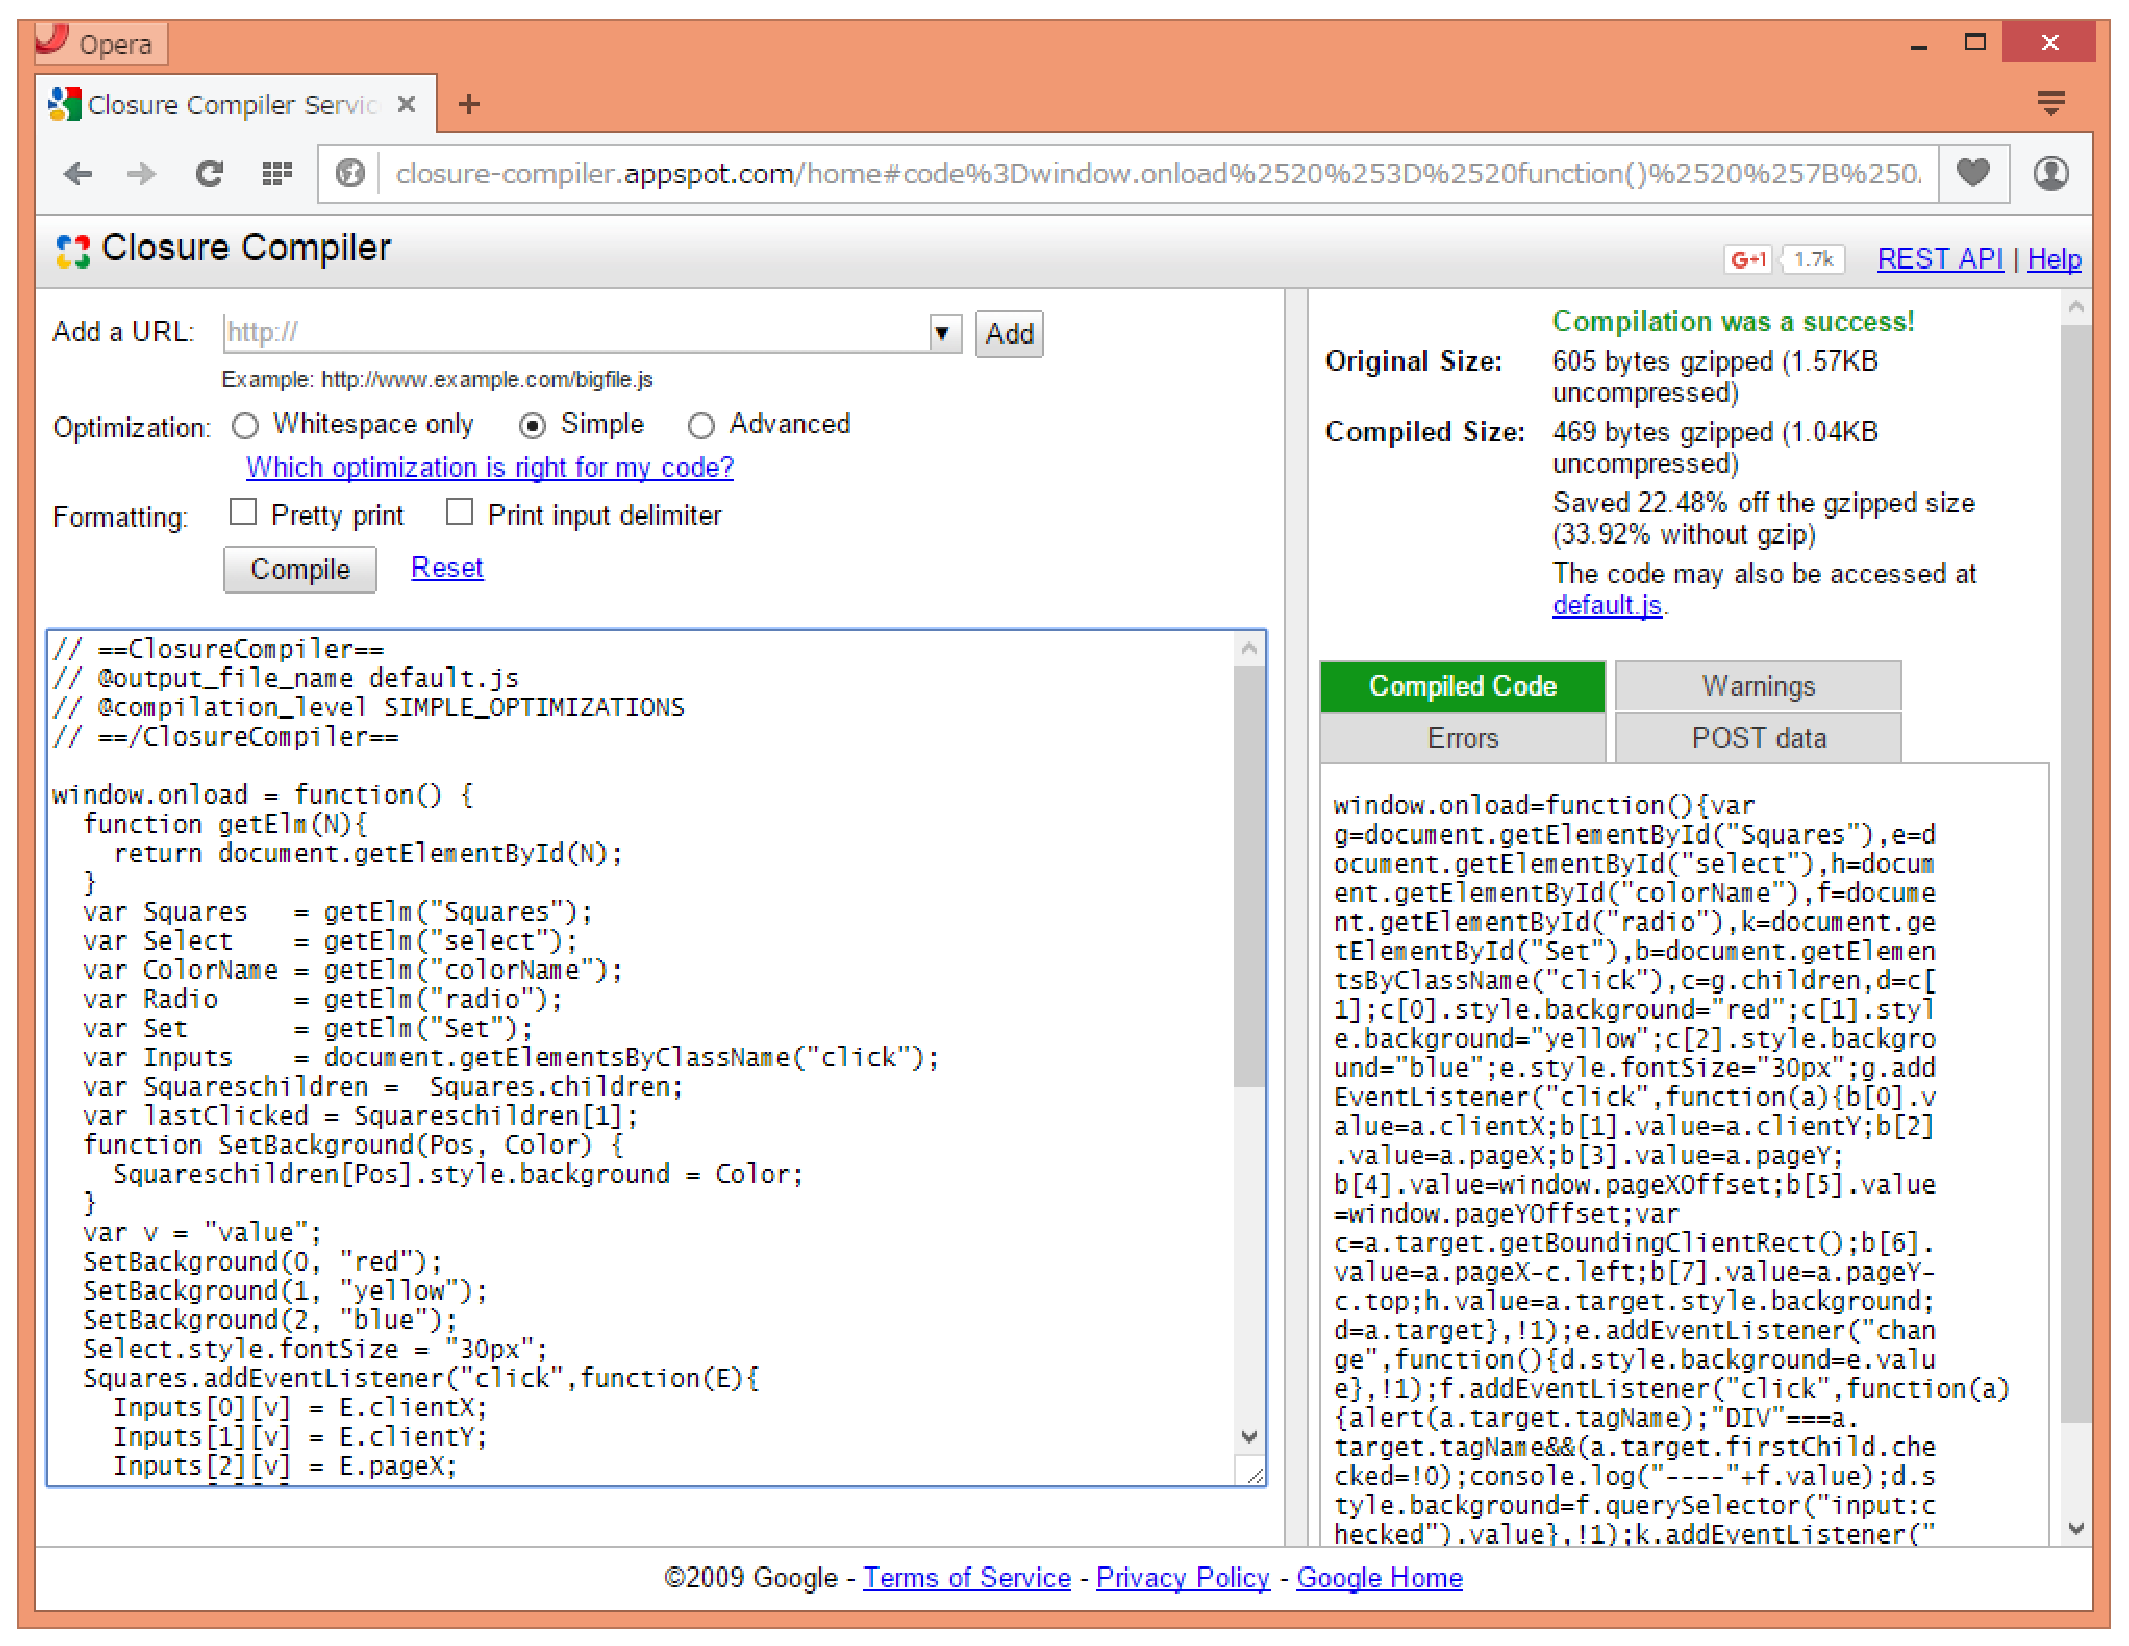
\includegraphics[width=1\textwidth]{../10-01closur-compiler-res02.eps}
	\end{center}
 \caption{Closure Compiler の結果(2)}\label{closure-compiler-res02}
 \end{figure}
\end{frame}
\begin{frame}[containsverbatim]
 \frametitle{解説}
ラップした関数は消えていて、もとの
 \texttt{document.getElementById}に戻っている。

 これを避けるためには関数を定義してその場で実行する関数の引数に
 \texttt{document}と\texttt{"getElementById"}を渡すことで解決できる。

 
\end{frame}
\begin{frame}[containsverbatim]
 \frametitle{ソースコードの書き直し(1)}
 {\small
\begin{verbatim}
  var Squares, Select, ColorName, Radio, Set;
		(function(document,getElementById){
      Squares   = document[getElementById]("Squares");
      Select    = document[getElementById]("select");
      ColorName = document[getElementById]("colorName");
      Radio     = document[getElementById]("radio");
      Set       = document[getElementById]("Set");
	})(document,"getElementById");
\end{verbatim}
}
\end{frame}
\begin{frame}[containsverbatim]
 \frametitle{ソースコードの書き直し(2)}
 \begin{figure}[ht]
	\begin{center}
	 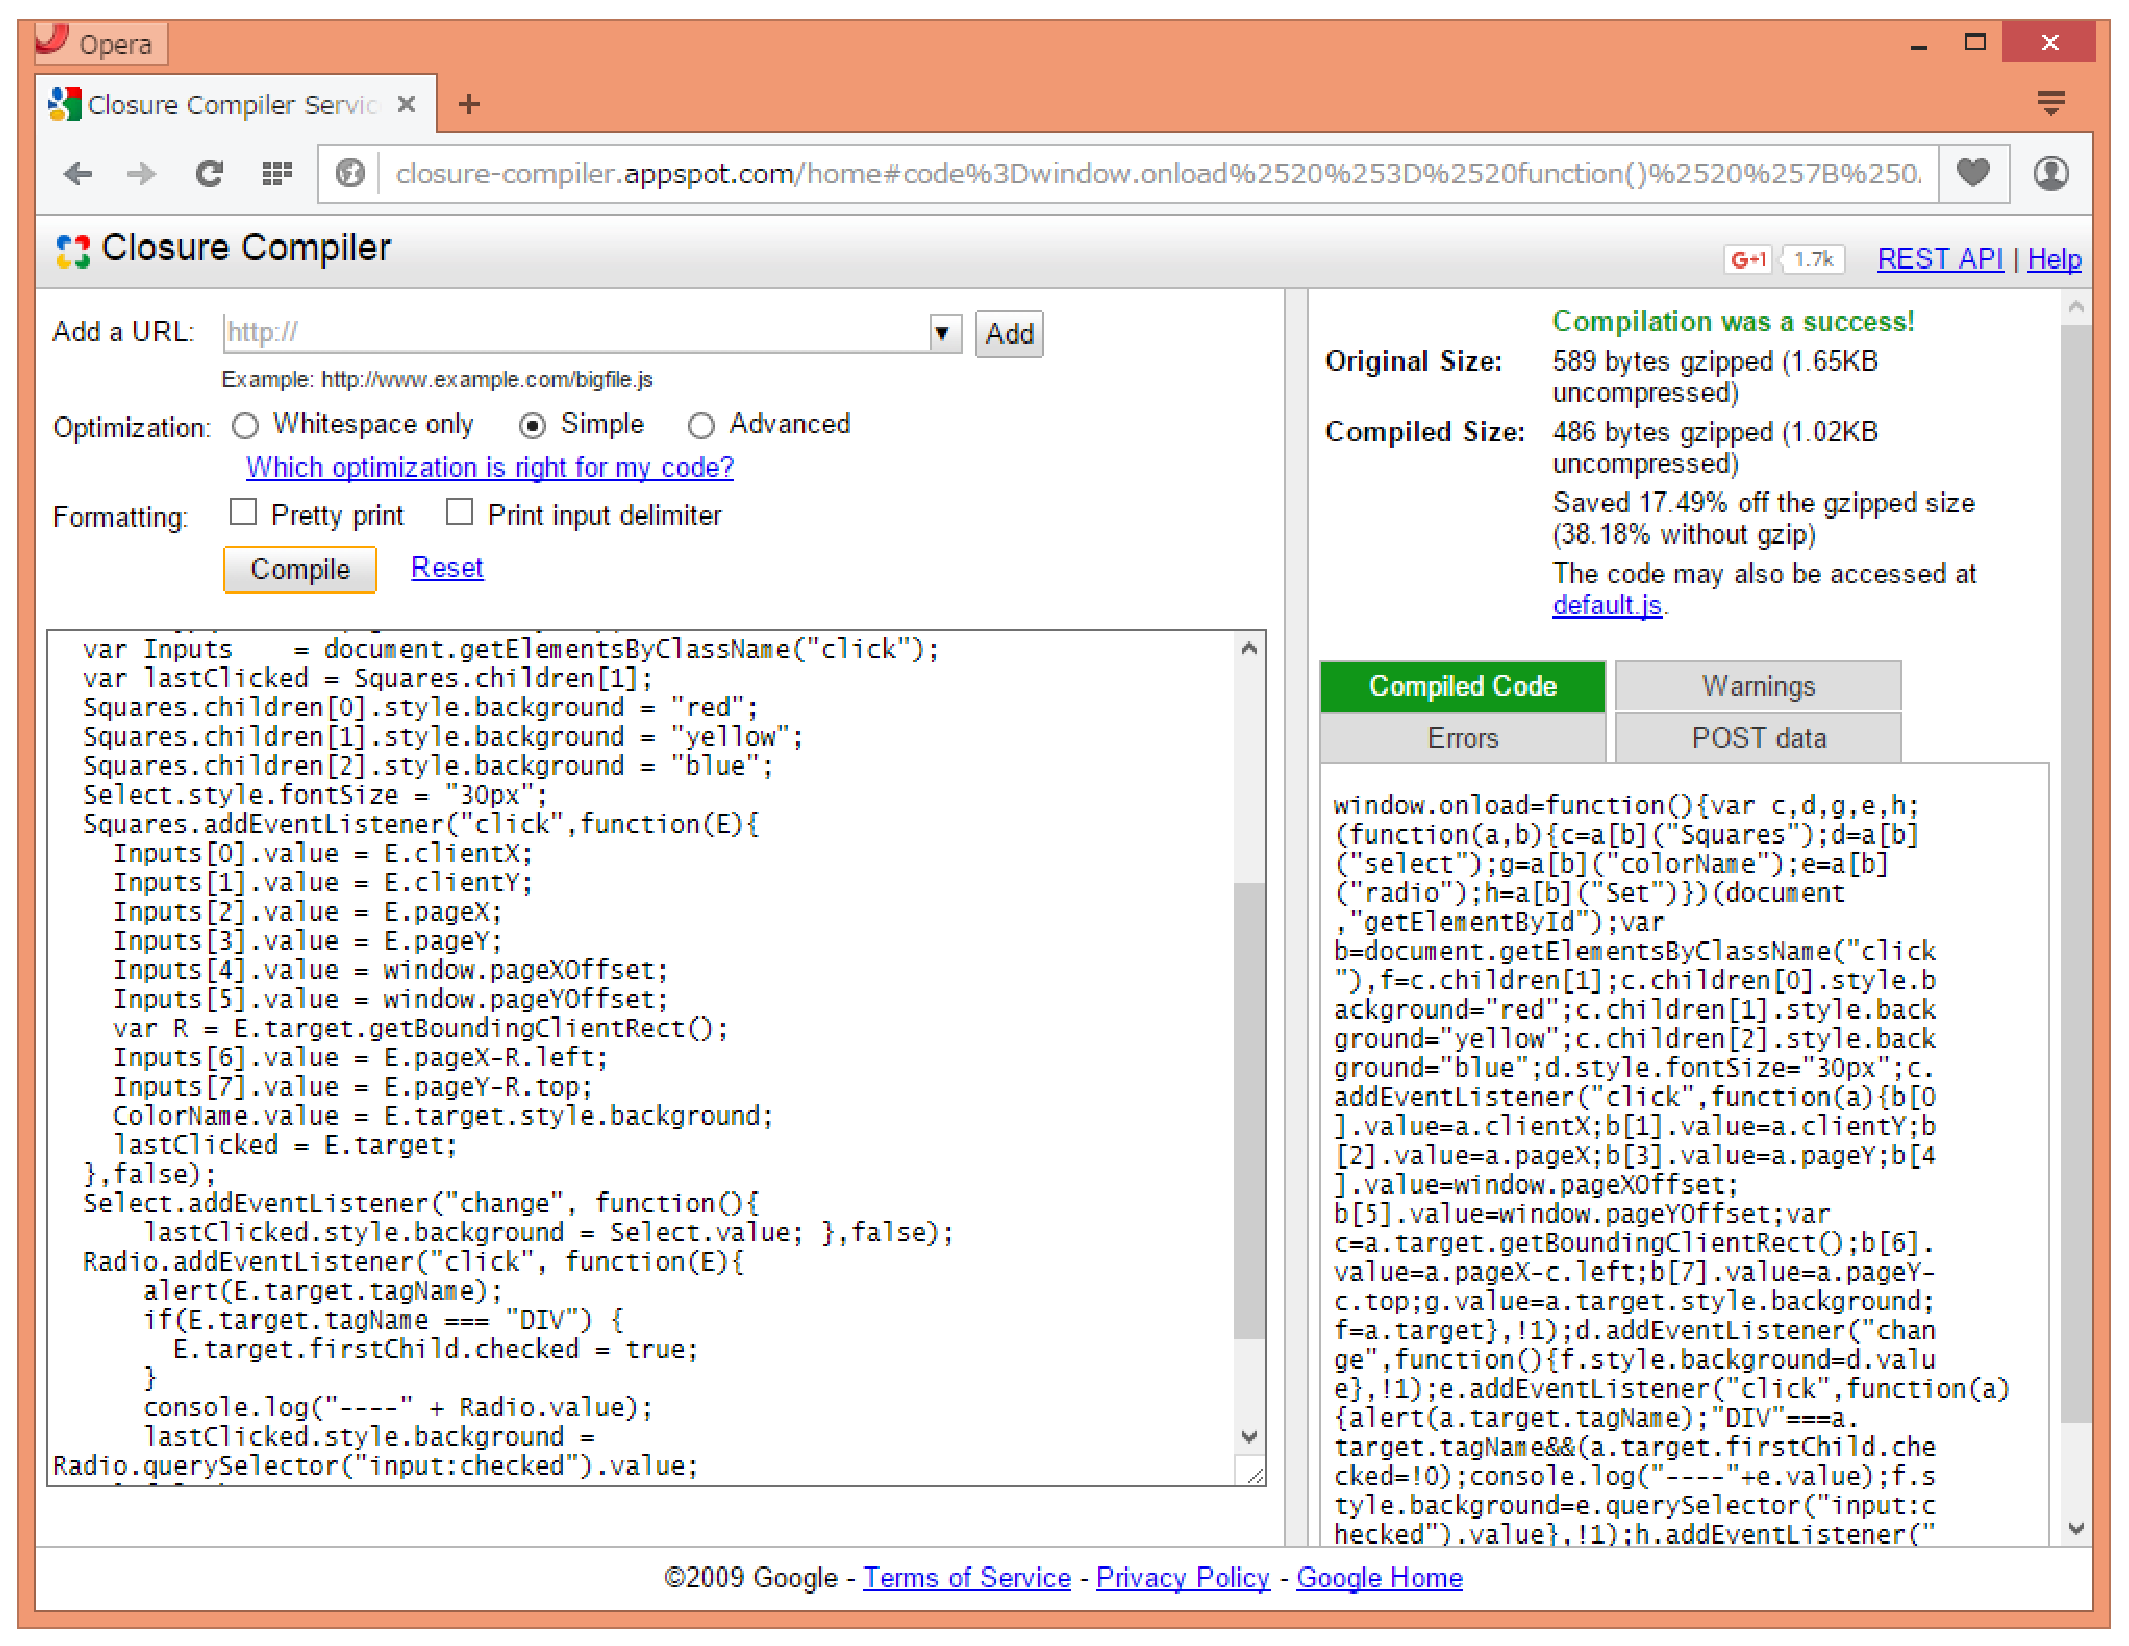
\includegraphics[width=1\textwidth]{../10-01closur-compiler-res03.eps}
	\end{center}
 \caption{Closure Compiler の結果(3)}\label{closure-compiler-res03}
 \end{figure}
\end{frame}
\begin{frame}[containsverbatim]
 \frametitle{ソースコードの書き直し(3)}
 コンパイル後の結果が1.02KBとわずかに小さくなっていることがわかる。

 短縮化を効率よくするためには元のプログラムも考えて作らないといけない。
\end{frame}
 \begin{frame}[containsverbatim]
\frametitle{注意}
この書き直しで\texttt{document.getElementById}だけを渡せば十分と思われるかもし
 れないが、これは関数オブジェクトとなり、関数内での\texttt{this}が
  \texttt{document}にならないので、実行時にエラーが生ずる。

与えられた関数を別のオブジェクトのメソッドとして実行するために、
  \texttt{call}メソッドを用いる。
\begin{verbatim}
  (function(document,getElementById){
      Squares   = getElementById.call(document,"Squares");
      Select    = getElementById.call(document,"select");
      ColorName = getElementById.call(document,"colorName");
      Radio     = getElementById.call(document,"radio");
      Set       = getElementById.call(document,"Set");
	})(document,document.getElementById);
\end{verbatim}
 \end{frame}
\end{document}
